\documentclass[10pt,a4paper,twoside]{article}
\usepackage[english]{babel}
%laad de pakketten nodig om wiskunde weer te geven :
\usepackage{amsmath,amssymb,amsfonts,textcomp}
%laad de pakketten voor figuren :
\usepackage{graphicx}
\usepackage{float,flafter}
\usepackage{hyperref}
\usepackage{inputenc}
\usepackage{minted}
\usepackage{subcaption}

\setlength\paperwidth{20.999cm}\setlength\paperheight{29.699cm}\setlength\voffset{-1in}\setlength\hoffset{-1in}\setlength\topmargin{1.499cm}\setlength\headheight{12pt}\setlength\headsep{0cm}\setlength\footskip{1.131cm}\setlength\textheight{25cm}\setlength\oddsidemargin{2.499cm}\setlength\textwidth{15.999cm}

\newcommand{\sweepsize}{0.26}

\begin{document}
\begin{center}
\hrule

\vspace{.4cm}
{\bf {\Huge Computer Vision} \\ {\huge Lab Assigment Report} \\ {\Large Local Features}}
\vspace{.2cm}
\end{center}
{\bf Tuan Mate Nguyen}  (tunguyen@student.ethz.ch)
\hrule



\section{Detection}
\subsection{Image gradients}

% Python code
%\begin{minted}[mathescape,
%    linenos,
%    numbersep=5pt,
%    gobble=2,
%    frame=lines,
%    framesep=2mm,
%    firstnumber=26]{csharp}
%\end{minted}

% Image
%\begin{figure}[H]
%    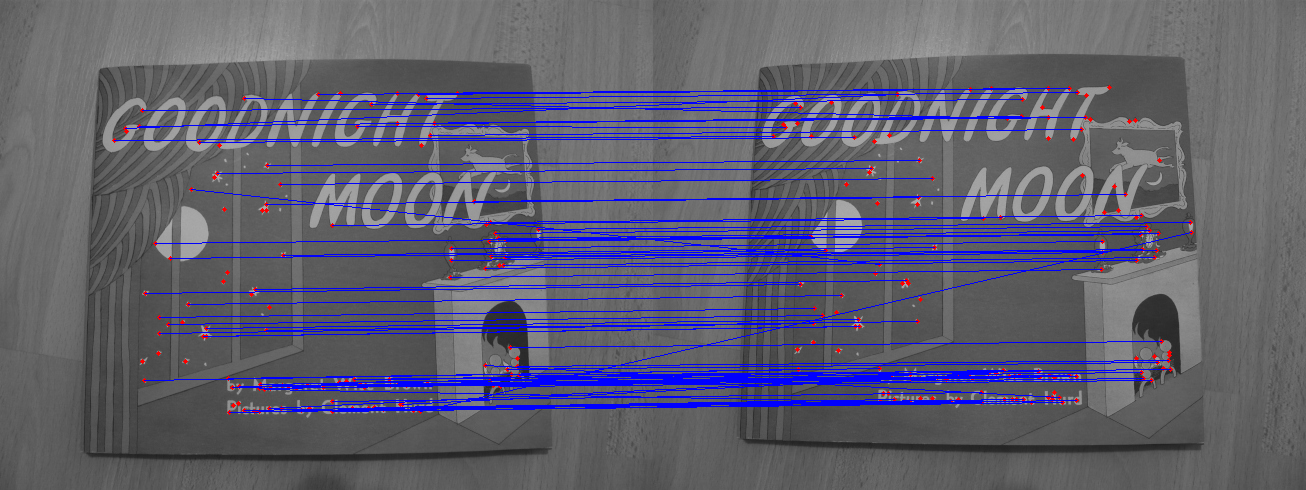
\includegraphics[width=\textwidth]{match_mutual.png}
%    \centering
%    \caption{Matching keypoints for mutual nearest neighbor matching}
%    \label{match_mutual}
%\end{figure}

\end{document}
